\documentclass{endm}
\usepackage{endmmacro}
\usepackage{graphicx}
\usepackage{amsmath}
\usepackage{caption}
\usepackage[brazilian,english]{babel}
\usepackage[utf8]{inputenc}
%\usepackage[T1]{fontenc}
\usepackage{multirow}

% The following is enclosed to allow easy detection of differences in
% ascii coding.
% Upper-case    A B C D E F G H I J K L M N O P Q R S T U V W X Y Z
% Lower-case    a b c d e f g h i j k l m n o p q r s t u v w x y z
% Digits        0 1 2 3 4 5 6 7 8 9
% Exclamation   !           Double quote "          Hash (number) #
% Dollar        $           Percent      %          Ampersand     &
% Acute accent  '           Left paren   (          Right paren   )
% Asterisk      *           Plus         +          Comma         ,
% Minus         -           Point        .          Solidus       /
% Colon         :           Semicolon    ;          Less than     <
% Equals        =           Greater than >          Question mark ?
% At            @           Left bracket [          Backslash     \
% Right bracket ]           Circumflex   ^          Underscore    _
% Grave accent  `           Left brace   {          Vertical bar  |
% Right brace   }           Tilde        ~

\newcommand{\Nat}{{\mathbb N}}
\newcommand{\Real}{{\mathbb R}}
\def\lastname{Brito}

\begin{document}  

% DO NOT REMOVE: Creates space for Elsevier logo, ScienceDirect logo
% and ENDM logo
\begin{verbatim}\end{verbatim}\vspace{2.5cm}

\begin{frontmatter}

\title{A Computational Study of Conflict Graphs and Aggressive Cut Separation in Integer Programming}
\author{Samuel Souza Brito \and Haroldo Gambini Santos\thanksref{mailSamuelHaroldo}}
\address{{\small Dep. de Computação, Universidade Federal de Ouro Preto - UFOP}}
\author{Marcus Poggi\thanksref{mailPoggi}}
\address{{\small Dep. de Informática, Pontifícia Universidade Católica do Rio de Janeiro}}
\thanks[mailSamuelHaroldo]{Email: {\texttt{\normalshape \{samuelsouza,haroldo\}@iceb.ufop.br}}} 
\thanks[mailPoggi]{Email: {\texttt{\normalshape poggi@inf.puc-rio.br}}}  

\begin{abstract}
This work explores the fast creation of densely populated conflict graphs at the root node of the search tree for integer programs. We show that not only the Generalized Upper Bound (GUB) constraints are useful for the fast detection of cliques: these can also be quickly detected in less structured constraints in $O( n \log n )$. Routines for the aggressive separation and lifting of cliques and odd-holes are proposed. Improved bounds and a faster convergence to strong bounds were observed when comparing to the default separation routines found in the current version of the COmputation INfrastructure for Operations Research (COIN-OR) Branch and Cut solver.
\end{abstract}

\begin{keyword}
conflict graphs, integer programming, cutting planes, cliques, odd-holes
\end{keyword}

\end{frontmatter}


\section{Introduction}\label{intro}

A conflict graph (CG) represents logical relations between binary variables. CGs are typically constructed using probing techniques~\cite{Savelsbergh1994} based on constraints analysis. On this work we propose an approach to speed up the creation of dense conflict graphs at the root node. Exact separation routines are employed to discover violated cliques and odd-holes, which are lifted in subsequent steps.

In Section~\ref{seccgraph} we formally explain our approach to speedup the detection of logical implications; in Section~\ref{cut} we present the cut separation and lifting routines; in Section~\ref{experiments} computational experiments are presented and finally, in Section~\ref{conclusions} we conclude and discuss the results of this work.

\section{Conflict Graphs in Integer Programming}\label{seccgraph}

A conflict graph represents logical relations between binary variables. Vertices represent variables and their complements, and edges indicate that two variables represented by the vertices must not be set to specific values without violating one or more constraints.

Given an Integer Program (IP), a conflict graph can be constructed using probing techniques based on feasibility considerations~\cite{atamturk}, checking the impact of fixing pairs of variables to different combinations of values. First, consider that each constraint $i \in \{1,\ldots,m\}$ can be written as $\displaystyle \sum_{j \in N} a_{ij}x_{j} \leq b_{i}$, where $N=\{1,\ldots,n\}$ is the index set of binary variables $x$, $a_{ij}$ is the coefficient for variable $x_{j}$ at constraint $i$ and $b_{i}$ is the right-hand side of constraint $i$.

Suppose we are analyzing two particular variables $x_j$ and $x_k$ with respect to constraint $i$. Consider that these variables are assigned with values $u$ and $v$, respectively. Consider also that $N_{i}^{-} = \{j \in N : a_{ij} < 0\}$. Then, $\displaystyle
L_{i}^{x_j = u,\, x_k = v}=\sum_{l\in N_{i}^{-} \setminus \{j, k\}}a_{il}+a_{ij}u+a_{ik}v $, is a lower bound for the value on the left-hand side of the constraint $i$, considering the assignments $x_j =u$ and $x_k=v$. If $L_{i}^{x_j = u,\, x_k = v} > b_{i}$, a conflict is detected for these assignments. 

Performing these steps considering each pair of variables in each constraint, leads to the creation of a conflict graph in $O(m \times n^2)$, where $m$ is the number of constraints and $n$ is the number of binary variables of the problem. Nevertheless, for some constraint types a large number of conflicts can be quickly discovered such as the Generalized Upper Bound constraints ($\displaystyle \sum_{j\in N}x_j \leq 1$). The following paragraphs describe the developed approach, which allows to detect cliques in individual constraints faster than $O(n^2)$. Notations $y_{ik}$ and $c_{ik}$ are used to indicate the variable with the $k$-th smallest coefficient in constraint $i$ and its coefficient. Constants $n_i$ and $S_i^-$ denote the number of non-zero variables and the sum of all negative coefficients of constraint $i$.

Conflicting variables can be detected just by traversing constraints with variables sorted in non-decreasing order of their coefficients. Thus, conflicts in these constraints are discovered in $O(n \log n)$. 

At first, consider that at a given position $k$ the summation of negative coefficients excluding the pair of variables at positions $k$ and $k+1$ in constraint $i$ is: $\displaystyle D_{i}\lbrack y_{ik}, y_{ik+1} \rbrack = S_i^- - min(0, c_{ik}) - min(0, c_{ik+1})$.  Thus, the lower bound for the LHS of constraint $i$ when variables with the $k-$th and $(k+1)-$th smallest coefficients are fixed at one is: $\displaystyle LHS_{i}\lbrack y_{ik} = 1, y_{ik+1} = 1 \rbrack = D_{i}\lbrack y_{ik}, y_{ik+1}\rbrack + c_{ik} + c_{ik+1}$.

Since this lower bound is monotonically non-decreasing as $k$ increases, if $\displaystyle LHS_{i}\lbrack y_{ik} = 1, y_{ik+1} = 1 \rbrack > b_{i}$, then there is a clique involving the activation of all variables from position $k$ until position $n_i$. Moreover, we can discard the existence of such cliques by checking if $\displaystyle LHS_{i}\lbrack y_{in_i-1} = 1, y_{in_i} = 1 \rbrack \leq b_i$.

Analogously, cliques involving complements of variables from positions $n_i$ until $k$ (i.e. traversing constraint $i$ in non-increasing order) can be obtained or discarded by calculating the limit incurred from positions $k$ and $k-1$: $\displaystyle LHS_{i}\lbrack y_{ik} = 0, y_{ik-1} = 0 \rbrack = D_{i}\lbrack y_{ik}, y_{ik-1}\rbrack$.

When the detected clique does not involve all variables of the analyzed constraint, a binary search is performed for each variable outside of the clique. Given a variable $y_{io}$ outside of the clique detected in $i$, binary search returns the first variable $y_{il}$ that has conflict with $y_{io}$. Thus, all variables from position $l$ to $n_i$ have conflict with $y_{io}$, forming another clique.

The developed approach can detect all conflicts involving original variables and also all cliques involving complements of variables. Conflicts involving both original and complements of variables are not discovered.

\section{Cutting Planes}\label{cut}

Linear programming relaxations can be significantly strengthened by the inclusion of inequalities derived from the Set Packing Polytope~\cite{Rebennack2009}. A clique inequality for a set $C$ of conflicting variables has the form $\displaystyle \sum_{j\in C}x_{j} \leq 1$ and an odd-hole inequality with conflicting variables $C$ can be defined as $\displaystyle \sum_{j\in C}x_{j} \leq \frac{|C|-1}{2}$.

Our proposed clique separation routine has two main components. The first of them is a module to separate \emph{all} violated cliques in the conflict subgraph induced by variables with fractional values at linear relaxation of root node. This module uses an improved version of the (exact) Bron-Kerbosch algorithm~\cite{Bron1973} that implements an optimized pivoting rule~\cite{Brito2011} to speed up the discovery of maximal cliques with large weight. The second component is a (heuristic) lifting module that considers the original conflict graph and iteratively tries to insert inactive variables, which are previously sorted in non-decreasing order of reduced cost. 

The developed odd-hole separation routine is the same used in~\cite{Rebennack2009}. The main idea is to construct an auxiliary bipartite graph from the original one and to search for shortest paths. We also heuristically lift the generated odd-holes, using strategy which is similar to used in the clique lifting. Iteratively, inactive variables previously sorted in non-decreasing order of reduced cost are selected and analyzed to be inserted in the generated odd-hole. A lifted odd-hole for variables $C$ and a wheel center $W$ can be written as: $\displaystyle \sum_{j \in W} \frac{|C|-1}{2} x_{j} + \sum_{j \in C} x_{j} \leq \frac{|C|-1}{2}$.

\section{Experimental Results}\label{experiments}

Our code was written using the open source COIN-OR \cite{LougeeHeimer2003} CLP libraries to solve linear programs and the CGL library was used to compare with our cut generation routines. All experiments ran on a computer with an Intel Core i7 3.6GHz processor and 32GB of RAM.

The first set of instances is the benchmark set of from MIPLIB 2010~\cite{miplib}, containing 87 instances. The second set of instances (INRC) comes from an IP formulation  used to solve the Nurse Rostering Problem~\cite{Santos2014} of the International Nurse Rostering Competition, containing 60 instances. Characteristics of each problem set are presented in Table~\ref{tab:inst}: columns ($n$), rows ($m$), non-zeros ($nz$). The notation ($\underline{v}$,$\overline{v}$,$\tilde{v}$) indicates minimum, maximum and average values.

The first experiment compares the construction of conflict graphs using pairwise detection ($PD$), which only detects cliques quickly in GUB constraints (conflicts in the remaining constraints are discovering by pairwise inspection), and our approach ($FCG$). Results are presented in Table~\ref{tab:graph}: number of edges ($|E|$) and total time in seconds spent in the construction of conflicts graphs for all instances of each set ($Time (sec)$). 

\begin{table}[htbp]
\scriptsize
\caption{Characteristics of instance sets.}
\begin{center}
\begin{tabular}{|l|c|c|c|c|r|r|}
\hline 
\multirow{2}{0.8cm}{\textbf{Inst. Set}} & \multicolumn{3}{c|}{{\textbf{Problem Sizes ($\times10^{3}$)}}} \tabularnewline
\cline{2-4} 
 & {$\underline{n}$/$\overline{n}$/$\tilde{n}$} & {$\underline{m}$/$\overline{m}$/$\tilde{m}$} & {$\underline{nz}$/$\overline{nz}$/$\tilde{nz}$} \tabularnewline
\hline 
\hline 
\texttt{MIPLIB} & {0.1/164.6/13.7} & {0.1/624.2/32.1} & {0.7/27678.7/515.9}\tabularnewline
\hline 
\texttt{INRC} & {9.8/63.6/29.7} & {3/29.2/11.7} & {201.1/1068.1/534.8}\tabularnewline
\hline 
\end{tabular}
\end{center}
\label{tab:inst}
\end{table}

\begin{table}[htbp]
\scriptsize
\caption{Comparison between pairwise detection and our approach.}
\begin{center}
\begin{tabular}{|l|r|r|r|r|}
\hline
\multirow{2}{0.8cm}{\textbf{Inst. Set}} & \multicolumn{ 2}{c|}{\textbf{PD}} & \multicolumn{ 2}{c|}{\textbf{FCG}} \\ \cline{ 2- 5}
\multicolumn{ 1}{|c|}{} & \multicolumn{1}{c|}{\textbf{$|\underline{E}|$/$|\overline{E}|$/$|\tilde{E}|$ ($\times10^{3}$)}} & \multicolumn{1}{c|}{\textbf{Time (sec)}} & \multicolumn{1}{c|}{\textbf{$|\underline{E}|$/$|\overline{E}|$/$|\tilde{E}|$ ($\times10^{3}$)}} & \multicolumn{1}{c|}{\textbf{Time (sec)}} \\ \hline
\texttt{MIPLIB} & 0/11396,11/480,82 & 173,37 & 0/11396,11/477,71 & 23,91 \\ \hline
\texttt{INRC} & 2470,14/12807,28/6346,36 & 370,4 & 2469,70/12803,68/6344,88 & 369,99 \\ \hline
\end{tabular}
\end{center}
\label{tab:graph}
\end{table}

The second experiment compares the cut generation routine of COIN-OR CGL (CGL) and our cut generation routines with (LNPSEP) and without lifting module (NPSEP). Figure~\ref{figExperiments} shows the average gap closed improvement for each instance set. After removing infeasible instances and instances where neither our code or CGL found any violated inequality, there were left 18 instances of MIPLIB and 60 of INRC set. The time limit was fixed in 150 seconds. While remarkable improvements in terms of bounds were obtained in the INRC instances (from 76.56\% with CGL to 84.76\% with LNPSEP), which have a large number of dense set partitioning and packing constraints, a modest improvement occurred in MIPLIB instances. The average gap closed for these instances was improved from 67.32\%, obtained with CGL, to 68.83\%, obtained with LNPSEP within the time limit imposed. 

\begin{figure}	
	\begin{minipage}[h]{.5\textwidth}
		\begin{center}
			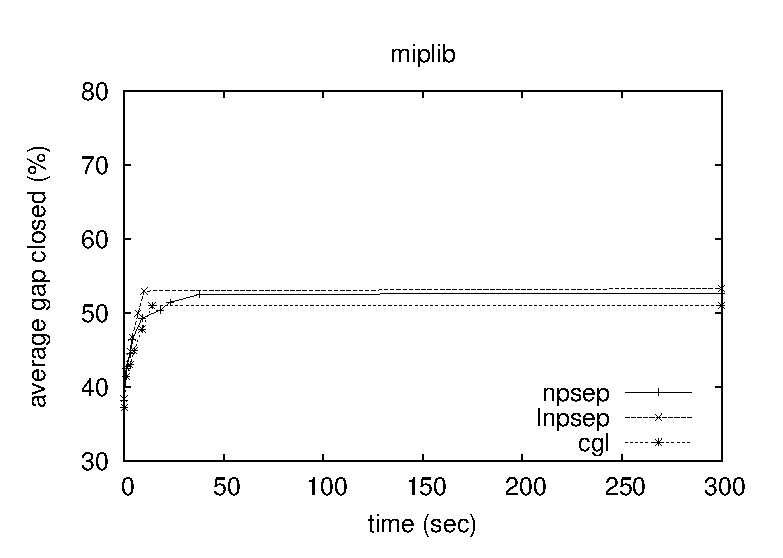
\includegraphics[width=1\textwidth]{miplib.eps}
		\end{center}
	\end{minipage}
	\begin{minipage}[h]{.5\textwidth}
		\begin{center}
			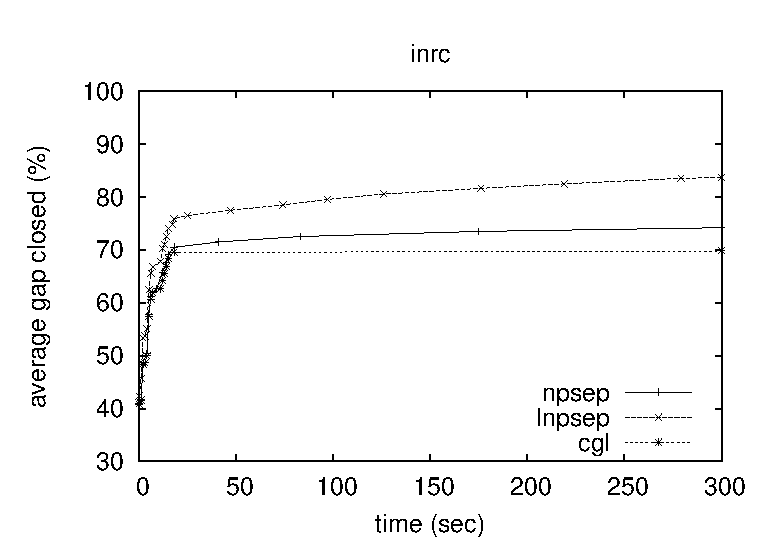
\includegraphics[width=1\textwidth]{nurse.eps}
		\end{center}
	\end{minipage}
	\caption{Dual bound improvement using LNPSEP, NPSEP and CGL routines.}
	\label{figExperiments}
\end{figure}

\section{Conclusions}\label{conclusions}

We developed an approach for fast creation of densely CGs using the detection of cliques in less structured constraints. A speedup of up to 7 times was obtained in the overall time to create an initial conflict graph. We also proposed and implemented a cut separation procedure. Experiments show that our cut generator can produce significantly better dual bounds than COIN-OR CGL, specially in restricted execution times. The source code of this work and detailed results of all experiments can be found on the project web page: \url{https://github.com/hgs/npsep/wiki}.

\bibliographystyle{endm}
\bibliography{references}

\end{document}
